\section{Results}
\label{sec:results}

% Ordered by the pillars of Sections 4 to 6; for each, what it was meant to establish, what was measured, what was
% found and why it matters for the claim (outline.md, Claim and contributions). Values come from the aggregate files of
% the main computation through make_tables.py. KeyTAR (A4) was moved to Appendix E on 29 October 2026;
% it is not part of the strongest attacker, so no statement on the other forms depends on it.
Values are for full texts and the 500 writers unless stated otherwise, in percent, with 95\% intervals in brackets;
no writer met an exclusion criterion. Every attacker at every $N$, the windows and the diagnostics are in
Appendix~\ref{app:results}.

\begin{table*}
  \caption{The strongest attacker on full texts, 500 writers. A0: accuracy of the total-length attacker. Strongest:
  accuracy of the best adaptive attacker with its interval; the selected attacker is given with the percentage of
  resamples in which it was selected when this is below 100. $\times 1/N$: the accuracy as a multiple of chance.
  Gain: the difference from A0 in percentage points. Measures: the numbers of the ten process measures computed with
  the same inputs as in R0, approximated and not computed; $\rho$: the median over the ten measures of the Spearman
  correlation with R0 (a measure not computed counts as zero). The measures do not depend on $N$. At 100\% the
  bootstrap interval is degenerate and does not show the uncertainty.}
  \label{tab:main}
  \small
  \setlength{\tabcolsep}{4pt}
  \begin{tabular}{lrlrrlrr}
    \toprule
    \multicolumn{8}{l}{(a) $N = 1{,}000$ ($1/N = 0.1\%$)} \\
    Form & A0 & Strongest & Attacker & $\times 1/N$ & Gain over A0 & Measures & $\rho$ \\
    \midrule
    \tabinput{sections/generated/main-1000.tex}
    \midrule
    \multicolumn{8}{l}{(b) $N = 10$ ($1/N = 10\%$)} \\
    Form & A0 & Strongest & Attacker & $\times 1/N$ & Gain over A0 & & \\
    \midrule
    \tabinput{sections/generated/main-10.tex}
    \bottomrule
  \end{tabular}
\end{table*}

\subsection{The masking of the public release}
\label{sec:results:masking}

This part asks whether the masking used in the competition (R1) keeps a log apart from its text, measured by the
strongest attacker's accuracy against $1/N$ and A0, with the negative control beside it. It does not, against the attacker that rebuilds the final draft as the winning solution did: on R1, A1 chose the
true text for every log in every draw, at $N = 1{,}000$ as at $N = 10$ (1,000 times $1/N$, a gain of 98.2 points
[97.1, 99.2] over A0, selected in every resample). R1 gave the same values as the unprocessed log R0, as did R5 and R6
(Appendix~\ref{app:results}), also for the 18 writers whose rebuilt draft differs from the distributed text. In the negative
control, the same attacker chose the true text in 0.0\% of draws at $N = 1{,}000$ and 9.9\% at $N = 10$, close to
$1/N$, so the accuracy comes from the link between each log and its own text; the open-world area was 1.000.

This is contribution C1. Under our reading of the stated goal (\S\ref{sec:threat-model:attacker}), the masking does
not keep a log apart from its text for anyone who holds the essays of the same prompt: the word lengths that the
masking leaves were enough to pick each essay out of a thousand.

\subsection{Forms that release less}
\label{sec:results:forms}

This part asks which columns carry the link, measured by the contrasts between adjacent forms
(\S\ref{sec:protocol:quantities}). Dropping the activity and the text change (R1~$-$~R2) changed little: A1 rebuilt
the draft from the categories and the position and reached 98.6\% [97.4, 99.6] at $N = 1{,}000$ (difference 1.4
points [0.4, 2.6]). Dropping the position and the word count as well (R2~$-$~R3) cost the strongest attacker 11.9
points [9.1, 15.1], but on R3 the editor replay A1$'$, which reads only the category column, still chose the true text
in 86.7\% [83.5, 89.5] of draws (867 times $1/N$). Rounding the press times did not change the strongest attacker for
any $w$, since A1$'$ does not use times; the timing attacker A3 fell from 47.1\% on R3 to 42.6\%, 40.7\% and 5.4\% at
$w = 10$, $100$ and $1{,}000$\,ms (differences 4.5 [2.4, 6.9], 6.4 [3.2, 9.8] and 41.7 [37.2, 46.1] points).

Merging the separators into one category (R3~$-$~R3-u) lowered the strongest attacker by 50.7 points [46.0, 55.1], to
36.0\% [31.9, 40.2], by A3 with its mean timing term. On R3-u, A0 counts all characters, separators included, and
reached 19.2\% by itself, so the gain over A0 is 16.8 points [13.6, 20.1]. Releasing only the segment values kept A2 at its value on R3 for $w =
1$ (40.5\% [36.1, 44.8]), lowered it to 4.4\% [2.8, 6.3] for $w = 2$, and for $w = 4$ and $8$ left no attacker above
A0. With the lighter penalty $\lambda = 4$, a registered secondary analysis (\S\ref{sec:attackers:alignment}), A2
reached 75.1\%, 36.4\% and 4.5\% for $w = 1$, $2$ and $4$, and on windows of 5 to 50 segments, at $N = 1{,}000$ with
$\lambda = 8$, A2 chose the true window in 44\% to 58\% of draws on R4(2) and 13\% to 43\% on R4(4) (Appendix~\ref{app:results}).
Suppression lowered the strongest
attacker to 70.2\% [66.0, 74.2], 14.3\% [11.5, 17.4] and 2.2\% [1.4, 3.4] for $p = 0.1$, $0.25$ and $0.5$; at $p =
0.5$ the strongest attacker was A0 (gain 0.0 [0.0, 1.1]).
The low full-text values on the coarse forms reflected the attackers. Two exploratory analyses decided after these
results (Appendix~\ref{app:exploratory}), A2 and A1$'$ with $\lambda$ from 2 to 16 and A2 aligning chunks of 20
segments anywhere in the text, raised the strongest attacker at $N = 1{,}000$ to 92.3\% [89.9, 94.5], 48.2\% [43.9,
52.4] and 2.4\% [1.3, 3.6] for $w = 2$, $4$ and $8$, and to 93.0\% and 62.3\% [58.1, 66.3] for $p = 0.1$ and $0.25$,
mostly with $\lambda = 2$, the lowest value tried; R7(0.5) stayed at A0.

At $N = 10$ the order of the forms is the same except that R3-u rises above R4(1) and R7(0.5) above R4(2), but A0 alone already chose the true text in 61.6\% of draws, so the
gains are smaller (Table~\ref{tab:main}b): 32.0 points on R3, 3.8 points [2.2, 5.4] on R3-u, and none whose lower
bound is above zero on R4($w$) and on R7 with $p \geq 0.25$, for attackers that do not combine A0 with the others
(\S\ref{sec:protocol:quantities}). The negative control stayed near $1/N$ for every form
(9.6\% to 11.5\% at $N = 10$, at most 0.34\% at $N = 1{,}000$).

This is the first axis of contribution C2. Against the attackers tried, the forms that keep the key categories (R2,
R3, R3-t) left matching within 14 points of the masking, and the times were not needed by the strongest attacker. Only
merging the separators, coarsening the segment values to $w \geq 2$ or suppressing at least a quarter of the presses
brought the strongest attacker below 40\% at $N = 1{,}000$, and only R4(4), R4(8) and R7(0.5) left no gain over the
total length (R4(4) not against A2 with $\lambda = 4$, and only R7(0.5) against the exploratory attackers). These contrasts contain the difference in attackers as well as in columns
(\S\ref{sec:threat-model:bias}).

\subsection{The cost to the process measures}
\label{sec:results:utility}

\begin{figure}
  \centering
  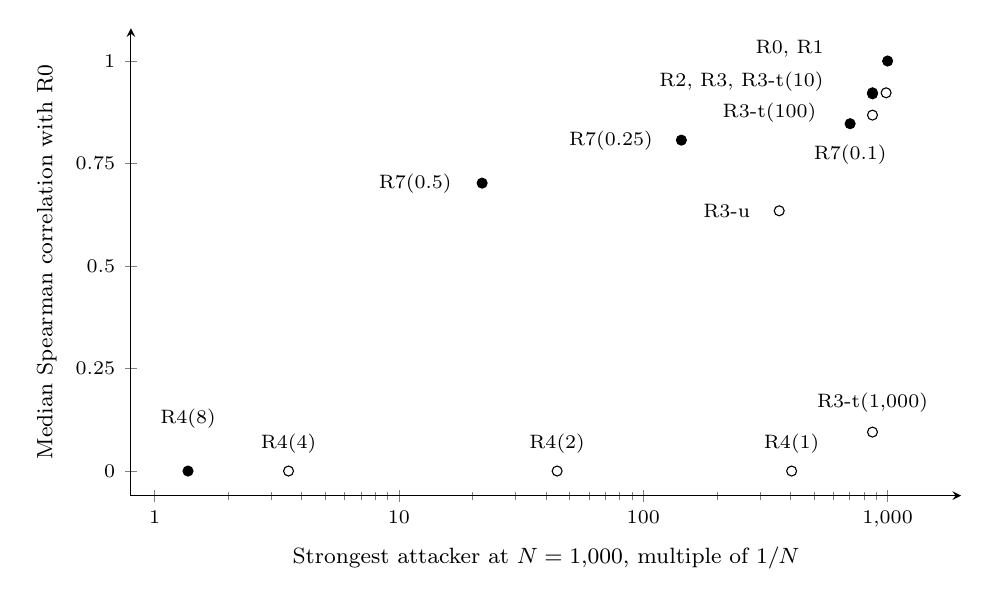
\begin{tikzpicture}
    \begin{semilogxaxis}[
      width=\linewidth, height=0.62\linewidth,
      xmin=0.8, xmax=2000, ymin=-0.06, ymax=1.08,
      xlabel={Strongest attacker at $N = 1{,}000$, multiple of $1/N$},
      ylabel={Median Spearman correlation with R0},
      tick label style={font=\scriptsize}, label style={font=\footnotesize},
      xtick={1,10,100,1000}, xticklabels={1,10,100,1{,}000},
      ytick={0,0.25,0.5,0.75,1}, axis lines=left,
    ]
      % Coordinates from sections/generated/figure-coords.tex. Filled: not dominated; open: dominated.
      \addplot[only marks, mark=*, mark size=1.8pt, black] coordinates
        {(1000,1.0) (867.2,0.9225) (702.4,0.8471) (143.2,0.8070) (21.9,0.7022) (1.37,0.0)};
      \addplot[only marks, mark=o, mark size=1.8pt, black] coordinates
        {(986,0.9225) (867.2,0.9200) (867.2,0.8681) (867.2,0.0950) (360,0.6347) (404.8,0.0) (44.4,0.0) (3.533,0.0)};
      \node[font=\scriptsize, anchor=east] at (axis cs:600,1.03) {R0, R1};
      \node[font=\scriptsize, anchor=east] at (axis cs:600,0.95) {R2, R3, R3-t(10)};
      \node[font=\scriptsize, anchor=east] at (axis cs:560,0.875) {R3-t(100)};
      \node[font=\scriptsize, anchor=north] at (axis cs:702.4,0.82) {R7(0.1)};
      \node[font=\scriptsize, anchor=east] at (axis cs:120,0.807) {R7(0.25)};
      \node[font=\scriptsize, anchor=east] at (axis cs:18,0.702) {R7(0.5)};
      \node[font=\scriptsize, anchor=east] at (axis cs:300,0.635) {R3-u};
      \node[font=\scriptsize, anchor=south] at (axis cs:867.2,0.12) {R3-t(1{,}000)};
      \node[font=\scriptsize, anchor=south] at (axis cs:404.8,0.02) {R4(1)};
      \node[font=\scriptsize, anchor=south] at (axis cs:44.4,0.02) {R4(2)};
      \node[font=\scriptsize, anchor=south] at (axis cs:3.533,0.02) {R4(4)};
      \node[font=\scriptsize, anchor=south] at (axis cs:1.37,0.08) {R4(8)};
    \end{semilogxaxis}
  \end{tikzpicture}
  \caption{No form evaluated brought matching near chance while computing the process measures. Matching against the
  measures for the main forms, full texts, $N = 1{,}000$, attackers with $\lambda = 8$ (lower left: less matching, fewer
  measures); the utility axis has no interval, so dominance by a small difference rests on the point estimates. Filled: forms that no other form dominates, that is, no other form has a lower or equal
  accuracy and a higher or equal correlation, one of them strictly. Open: dominated forms.}
  \label{fig:tradeoff}
\end{figure}

This part asks what each form costs writing research, measured by the agreement of the ten process measures with
their values in R0 (\S\ref{sec:protocol:utility}). R0 and R1 compute all ten measures as before. R2 and R3 compute the
P-bursts, the pauses and the variance of the production rate as in R0 and approximate the R-bursts, deletions and
insertions, with correlations from 0.19 (insertion proportion) to 0.85 (deletion proportion); with the five measures
computed as in R0, the median is 0.92. The approximation rules do not use the position column of R2, so R2 has the
values of R3. At $w = 1{,}000$\,ms five measures cannot be computed,
R3-u loses the pauses within and between words, and R4 computes none (Table~\ref{tab:main}).

Figure~\ref{fig:tradeoff} plots the two axes. The forms that no other form dominates are R0 and R1, R3, the three
levels of suppression and R4(8). R3 dominates R2 and R3-t, which have the same or a lower correlation and the same
accuracy or a higher one, and R7(0.25) dominates R3-u, with a lower accuracy (14.3\% against 36.0\%) and a higher
correlation (0.81 against 0.63). The approximations also change how a
measure relates to the human scores: the mean pause correlates with the score at $-0.11$ in R0 and at $-0.50$ in
R7(0.5), and the R-burst length at $-0.04$ in R0 and at $0.20$ in R2 (Appendix~\ref{app:results}). The utility axis
measures agreement with R0, not whether a measure keeps its relation to the quality of writing.

This is the second axis of contribution C2, read from the forms that no other form dominates. R3 kept 86.7\% with
five measures as in R0 and a median correlation of 0.92; suppressing a tenth, a quarter and a half of the presses gave
70.2\%, 14.3\% and 2.2\% with medians of 0.85, 0.81 and 0.70; R4(8) gave 0.14\% and no measure. Only R4(4) and R4(8)
brought the strongest attacker within four times $1/N$, and they compute no measure; against the exploratory
attackers no form did (\S\ref{sec:results:forms}). Every main form from R2 on computed
the R-burst and insertion measures at a mean correlation below 0.5 or not at all (Appendix~\ref{app:results}).

\subsection{Windows and the open world}
\label{sec:results:windows}

This part asks whether releasing parts of logs changes the picture, and how well the scores separate candidate sets
with and without the true text. On windows, where A1 and A1$'$ are not run, A2 was the strongest attacker on R0 to R3,
R3-t and R4(1), with the same values on all of them, since A2 reads only the segments. At $N = 1{,}000$ it chose the
true window in 65.8\% [63.9, 67.8] of draws with $k = 5$ and in 72.3\% [70.2, 74.5] with $k = 20$; at $N = 10$, in 84\%
to 88\%. On R3-u, where A0 was the strongest attacker, accuracy at $N = 1{,}000$ was 0.6\% to 1.9\%; on R7(0.1), 26.7\%
to 47.5\%; on R4(8), 1.5\% to 16.7\% (Appendix~\ref{app:results}). Each decoy contributed one window, so these values
hold for far fewer candidates than an attacker searching every position of every text would face
(\S\ref{sec:threat-model:bias}), and no process measure is defined on windows.

In the open-world diagnostic, the area was 1.000 for R0 and R1, 0.978 for R2, 0.774 [0.753, 0.795] for R3 and R3-t
and at most 0.62 for the other forms. Within each log, a large margin between the best and the second-best candidate
marked correct matches: on R3, the 80\% of logs and draws with the largest margins were all matched correctly
(exploratory; Appendix~\ref{app:exploratory}). KeyTAR, the reference outside the threat model, stayed
below A0 on every form and $N$ (Appendix~\ref{app:results}).

\subsection{The Japanese translation logs}
\label{sec:results:enja}

This part asks question 4: whether the same kind of matching exceeds chance and A0 on logs typed with an input method,
measured by A2 on R3j at $N$ = all (\S\ref{sec:protocol:enja}). No session met an exclusion criterion, so all 76
sessions of 39 translators on six source texts were used, with 12 or 13 candidates per log. On R3j, which keeps no
string, A2 chose the true translation in 51.6\% [39.3, 63.5] of logs, against $1/N$ = 7.9\% and 11.9\% [5.3, 19.7] for
A0 (means over the six source texts). The differences were 43.7 points [31.4, 55.6] from $1/N$ and 39.7 points [25.6, 53.0] from A0; both lower bounds
are above zero, so by the registered rule matching exceeds chance and A0. Accuracy ranged from 33\% to
77\% over the source texts, and R3j-t($w$) and R4($w$) also exceeded both (Appendix~\ref{app:enja}); A2 reads the same
segments from R3j, R3j-t($w$) and R4(1), so these share its values. The result is
conditional (\S\ref{sec:discussion:limits}): without any string, the categories of input-method events kept enough
of a translation's segment structure to choose it in half of the logs.

\subsection{Exploratory analyses}
\label{sec:results:exploratory}

The exploratory analyses (\S\ref{sec:protocol:exploratory}) are reported in Appendix~\ref{app:exploratory}. Among
them, on R4(2) and R7(0.5) the matches concentrated on 4.2\% and 1.6\% of writers, matched in every draw, and accuracy
differed by score band on R3-u and on several coarse forms.
